%%%%%%%%%%%%%%%%%%%%%%%%%%%%%%%%%%%%%%%%%%%%%%%%%%%%%%
% Thanks to Xu Minghao's work                        %
% I modify it into uchicago version                  %
% to not make new bug, I don't alter "Ritsumeikan"   %
% keywords in file. Pls feel free to use             %
%%%%%%%%%%%%%%%%%%%%%%%%%%%%%%%%%%%%%%%%%%%%%%%%%%%%%%

%%%%%%%%%%%%%%%%%%%%%%%%%%%%%%%%%%%%%%%%%%%%%%%%%%%%%%
% A Beamer template for Ritsumeikan University       %
% Author: Ming-Hao Xu (Xu Minghao)                   %
% Date:   April 2022.                                %
% LPPL Licensed.                                     %
%%%%%%%%%%%%%%%%%%%%%%%%%%%%%%%%%%%%%%%%%%%%%%%%%%%%%%

\documentclass[compress]{beamer}
\usepackage[utf8]{inputenc}
\usepackage[spanish]{babel}
\usepackage{amsmath}
\usepackage{amsfonts}
\usepackage{amssymb}
\usepackage{graphicx}
\usepackage{lipsum}
\usepackage{ragged2e}
\usepackage{hyperref}
\usepackage{float}
\usepackage{url}
\usepackage{multicol}
\usepackage{subfigure}

\usetheme{Berlin}
\useoutertheme{miniframes}
\setbeamertemplate{navigation symbols}{} 


\newcommand{\celda}[1]{
	\begin{minipage}{2.5cm}
		\vspace{5mm}
		#1
		\vspace{5mm}
	\end{minipage}
}

\author[Cristhian Moya Mota]{Cristhian Moya Mota}
\title[PE en Series Temporales]{Estudio sobre la Efectividad del Positional Encoding en Transformers para Series Temporales y Diseño de Mecanismos Adaptados}
\date{8 de septiembre de 2025} 

\logo{
\includegraphics[scale=0.04]{pic/logo}}
\institute[UGR]{
	\inst{}
	Tutor: Julián Luengo Martín\\Departamento de Ciencias de la Computación e Inteligencia Artificial\\
	\inst{ }
	Cotutor: Diego Jesús García Gil\\Departamento de Lenguajes y Sistemas Informáticos\\
	\vspace{2mm}	
}

\AtBeginSection[]
{
	\begin{frame}<beamer>{Contenido}
		\tableofcontents[currentsection,currentsubsection]
	\end{frame}
}


\begin{document}
	
	\begin{frame}
		\maketitle
	\end{frame}
	
	\begin{frame}{Contenido}
		\tableofcontents
	\end{frame}
	
	\setbeamerfont{footnote}{size=\tiny}
	\section{Introducción}
	
	\begin{frame}{Introducción}
		\begin{figure}
			\centering
			\begin{minipage}{0.4\textwidth}
				\centering
				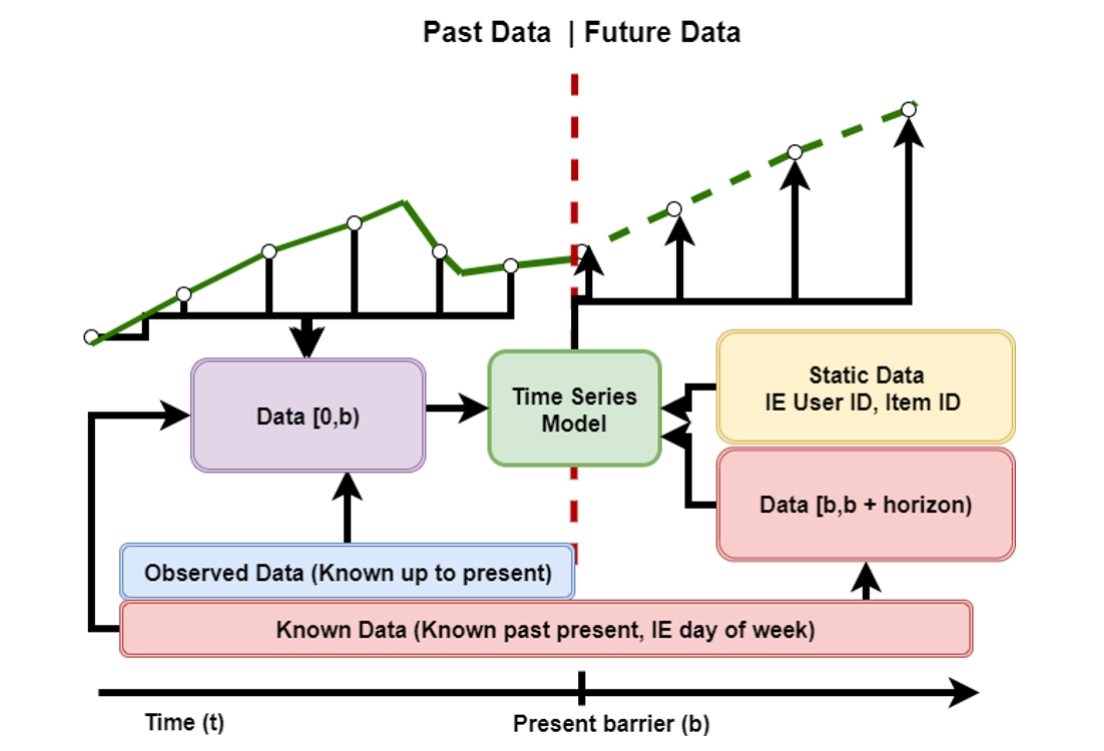
\includegraphics[height=\columnwidth]{pic/ts.png}
			\end{minipage}
			\hfill
			\begin{minipage}{0.4\textwidth}
				\centering
				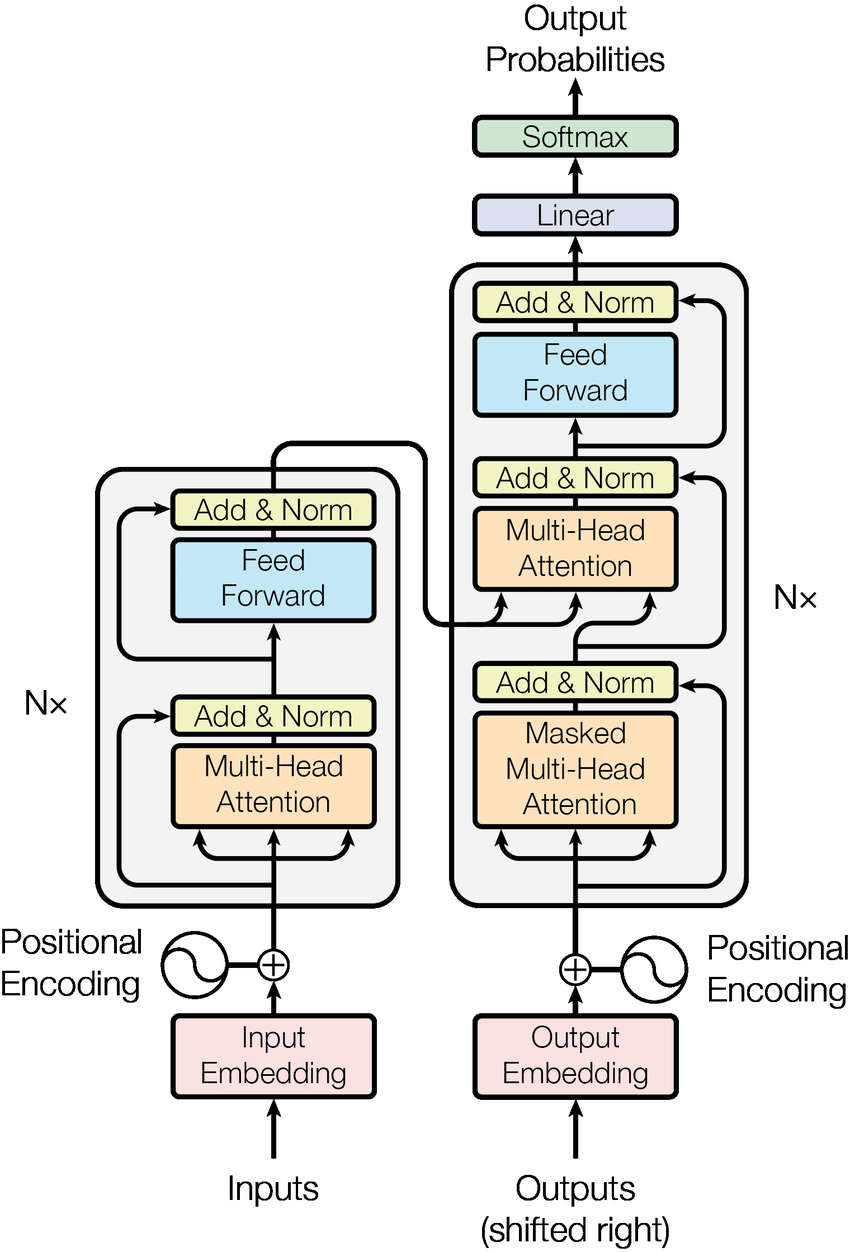
\includegraphics[height=\columnwidth]{pic/trans.png}
			\end{minipage}
			\caption[]{Forecasting en Series Temporales\footnote{{https://developer.nvidia.com/blog/time-series-forecasting-with-the-nvidia-time-series-prediction-platform-and-triton-inference-server/}}. Transformers\footnote{
					\url{https://doi.org/10.48550/arXiv.1706.03762}}}
		\end{figure}
	\end{frame}
	
	\begin{frame}{Introducción. Justificación}
		
		Aspectos que justifican la realización del proyecto:
		\begin{itemize}
			\item Falta de captura de la estructura. Ausencia de información semántica.
			\item Dificultad para adaptarse a diferentes escalas temporales y falta de semántica.
			\item Complejidad computacional y falta de interpretabilidad en la metodología.
		\end{itemize}
	\end{frame}
	
	\begin{frame}{Introducción. Objetivos}
		Este proyecto persigue:
		\begin{itemize}
			\item Comprender y exhibir las carencias de los métodos actuales.
			\item Proponer nuevos encodings para series temporales empleando Transformers.
			\item Evaluar la efectividad de las nuevas propuestas en diferentes ámbitos y conjuntos de datos.
			\item Identificar y establecer la base para nuevos métodos de codificación.
		\end{itemize}
	\end{frame}
	
	\section{Estado del arte}
	
	\begin{frame}{Estado del arte. Arquitecturas y PE}
		\begin{itemize}
			\item Métodos estadísticos: STL, ARIMA, Prophet.
			 
			\item Métodos basados en Transformer:
		
			\begin{itemize}
				\item Informer
				\item Autoformer
				\item FEDformer
			\end{itemize}
		\end{itemize}
		
		Problemas:
		\begin{enumerate}
			\item Escasa adición de información local.
			\item Mecanismos de atención poco cercanos a la semántica del dato.
		\end{enumerate}
		¿Solución? $\rightarrow$ Crear una nueva familia de codificaciones posicionales, capaz de captar información local y global.
	\end{frame}	 	
	\begin{frame}{Estado del arte. Caso particular de Informer}
		\begin{figure}
			\centering
			\begin{minipage}{0.55\textwidth}
				\centering
				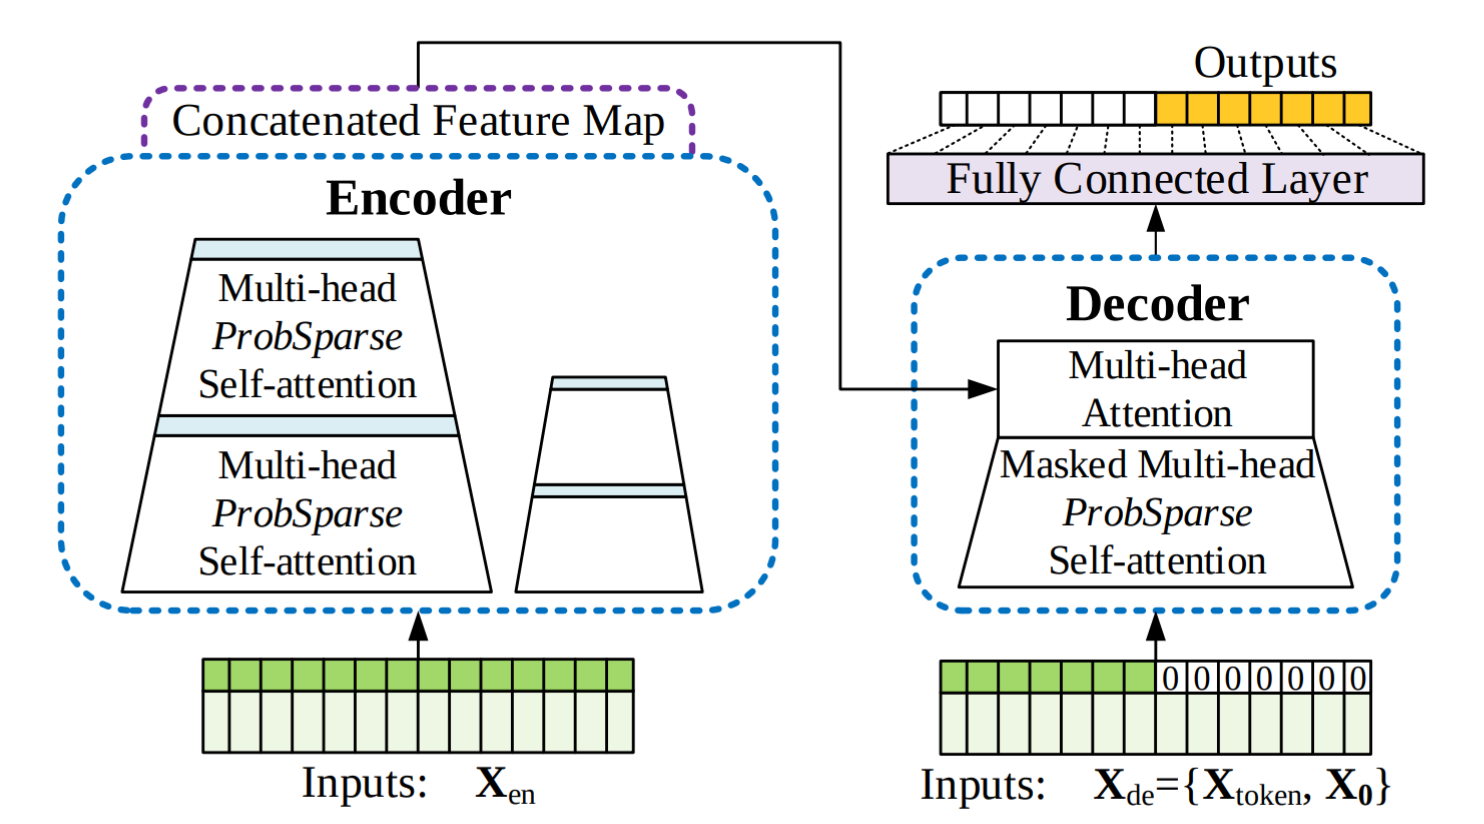
\includegraphics[width=\linewidth]{pic/informer.png}
			\end{minipage}
			\hfill
			\begin{minipage}{0.42\textwidth}
				\centering
				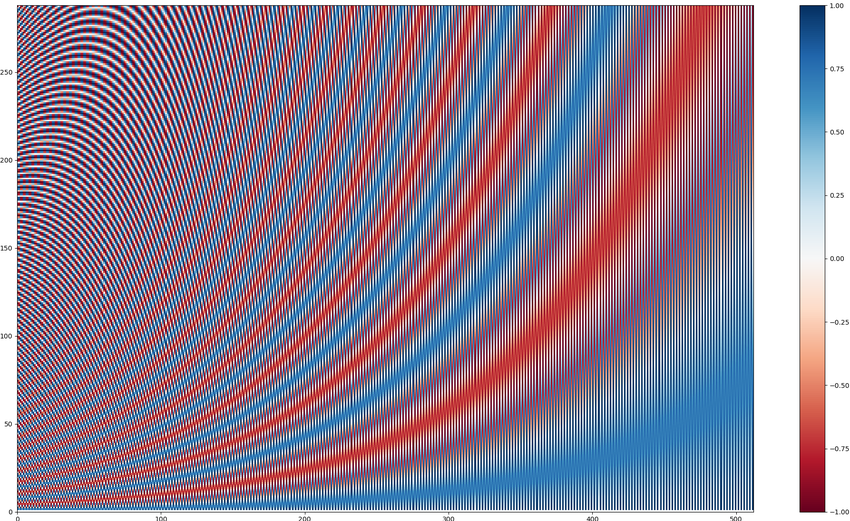
\includegraphics[width=\linewidth]{pic/encd}
			\end{minipage}
			\caption{Informer: arquitectura y encoding empleado\footnote{
					\url{https://doi.org/10.48550/arXiv.2012.07436}}}
		\end{figure}
	
	\end{frame}	 
		
	\section{Propuestas de positional encoding}
	\begin{frame}{Encodings propuestos: Aspectos clave}
		Para mejorar la calidad del encoding, hay dos alternativas:
		\begin{itemize}
			\item Modificar el mecanismo de atención $\rightarrow$ pérdida de información local y complejidad añadida
			\item Modificar únicamente el PE $\rightarrow$ permite aprovechar arquitecturas existentes y trabajar directamente sobre el dato
		\end{itemize}
		
		Resultado: familia de modelos WinStat:
		\begin{enumerate}
			\item Sólo modificar la codificación posicional
			\item Concatenar información en lugar únicamente sumarla
			\item Combinar PE existentes de manera ponderada (normalizada con Softmax):
			
			$$X_{\text{final}} \gets \tilde{w}_0 \cdot \tilde{X} + \tilde{w}_1 \cdot X_{pe1} + \tilde{w}_2 \cdot X_{pe2} + \tilde{w}_3 \cdot X_{pe3}$$
			
			 \end{enumerate}
	\end{frame}
	
	\begin{frame}{Encodings propuestos: WinStat (Variante base)}
	Ventana local de tamaño $W$ fijo, en cada posición $t$:
	
	\begin{itemize}
		\item \textit{Media}: $\mu_t = \frac{1}{|\mathcal{W}_t|} \sum_{x \in \mathcal{W}_t} x$
		\item \textit{Desviación estándar}: $\sigma_t = \sqrt{ \frac{1}{|\mathcal{W}_t|} \sum_{x \in \mathcal{W}_t} (x - \mu_t)^2 }$
		\item \textit{Mínimo}: $m^{\min}_t = \min_{x \in \mathcal{W}_t} x$
		\item \textit{Máximo}: $m^{\max}_t = \max_{x \in \mathcal{W}_t} x$
	\end{itemize}
	
	\[
	s_t = [\,\mu_t,\, \sigma_t,\, m^{\min}_t,\, m^{\max}_t\,] \in \mathbb{R}^{4}
	\]
	
	Y, finalmente, el embedding enriquecido de la posición $t$ es:
	
	\[
	\tilde{x}_t = [\,x_t \, \| \, s_t\,] \in \mathbb{R}^{d+4}
	\]
	
	\end{frame}
	
	\begin{frame}{Encodings propuestos: WinStatLag}
		
	Parte de WinStat, añadiendo $|\mathcal{L}|$ retardos especificados:
	
	\[
	s_t = [\,\mu_t,\, \sigma_t,\, m^{\min}_t,\, m^{\max}_t\,] \in \mathbb{R}^4
	\]
	
	Definimos para cada $\ell_j \in \mathcal{L}$:
	\[
	\delta_t^{(\ell_j)} = | x_t - x_{t - \ell_j}|, \quad \text{si } t - \ell_j \geq 1
	\]
	
	El \textit{embedding} enriquecido es la concatenaciçon de $s_t$ y $\delta_t^{(\ell_j)}$
	\[
	\tilde{x}_t = [\,x_t \,\|\, s_t \,\|\, \delta_t^{(\ell_1)} \,\|\, \dots \,\|\, \delta_t^{(\ell_p)}\,] \in \mathbb{R}^{d + 4 + p}
	\]

	
	\end{frame}
	
	
	\begin{frame}{Encodings propuestos: WinStatFlex}
		
	Basado en WinStatLags, añadiendo la información ponderada de:
	\begin{enumerate}
	\item Encoding sinusoidal original
	\item LPE:
	
	$$
	LPE_{(pos)} = W_{pos}, \quad W_{pos} \in \mathbb{R}^d
	$$
	
	$$
	X_{LPE} = \tilde{x}_t + LPE[pos]
	$$
	
	\item TAPE:
	
	\begin{equation}
		\centering
		\omega^{new}_k = k \cdot \frac{d_{model}}{L}
	\end{equation}
	
	
	\begin{equation}
		\begin{aligned}
			\text{TAPE}_{(pos,2i)} &= \sin\!\left( pos \cdot \omega^{new}_i \right) \\
			\text{TAPE}_{(pos,2i+1)} &= \cos\!\left( pos \cdot \omega^{new}_i \right)
		\end{aligned}
	\end{equation}
	
	$$
	X_{TAPE} = \tilde{x}_t + TAPE[pos]
	$$
	
		\end{enumerate}
	\end{frame}
	
	\begin{frame}{Encodings propuestos: WinStatTPE}
	\begin{itemize}
		\item Emplea WinStatFlex como base
		\item Sustituye TAPE por TPE:
		
		$$S(i, j) = \exp\left( -\frac{\|x_i - x_j\|^2}{2\sigma^2} \right)$$
		
		Añadiéndose al encoding sinusoidal original la nueva componente:
		
		$$T\text{-}PE(i) = PE(i) + S(i, j)$$
		
		$$
		X_{TPE} = \tilde{x}_t + T-PE[pos]
		$$
		
		
	 \end{itemize}
	\end{frame}
	
	\section{Evaluación de los PE mediante conjuntos de datos}
	
	\begin{frame}{Evaluación. Conjuntos de datos}
		Conjuntos de datos para la evaluación:
		
		\begin{columns}
			
			\column{0.4\linewidth}
			\begin{itemize}
				\item Household Power Consumption (HPC)
				\item ETTh1
				\item ETTh2
				\item Yellow Trip Data
				\item TINA
			\end{itemize}
		
			\column{0.6\linewidth}
			\centering
			\begin{figure}
				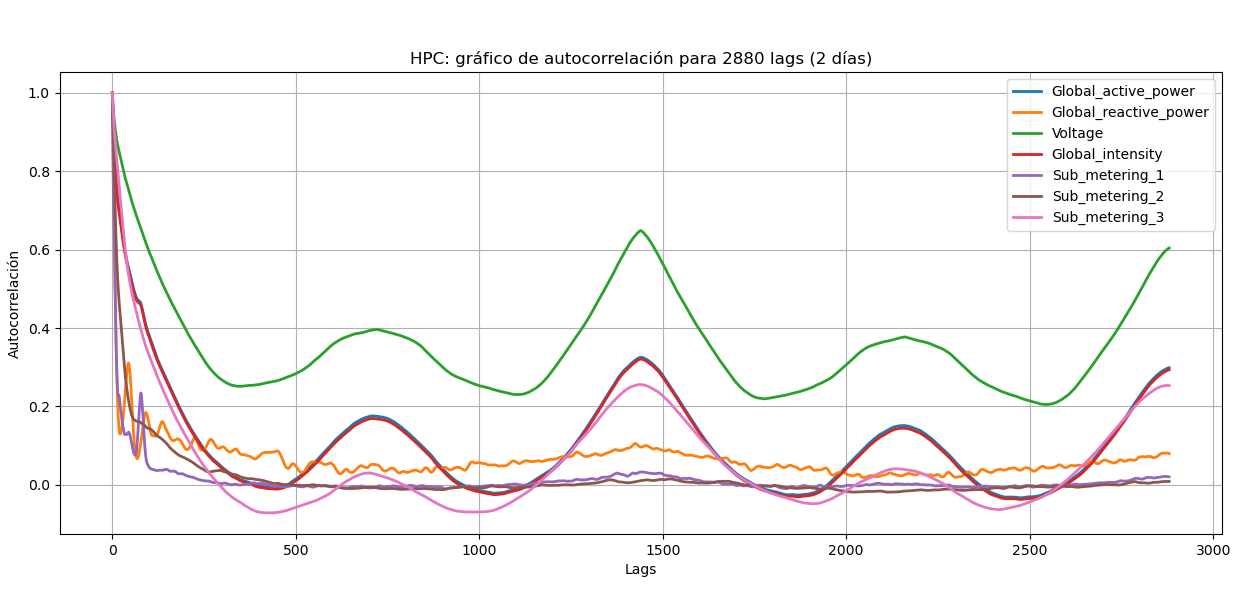
\includegraphics[width=\linewidth]{pic/auto.png}
				\caption{Autocorrelación de Household Power Consumption}
			\end{figure}
		
		\end{columns} 
				
	\end{frame}	

\section{Conclusiones y trabajos futuros}
\subsection{Conclusiones}
\begin{frame}{}
		El proyecto ha conseguido:
	
\end{frame}


\subsection{Trabajos futuros}
\begin{frame}{}
	\
\end{frame}


\begin{frame}
	\centering \textbf{Gracias}

	\begin{figure}[H,font=\Small]
		\centering
		\subfigure{
\includegraphics[width=0.2\textwidth]{pic/QRTFM}} 
		\label{fig:calidad}
		
		¿Preguntas?
		
	\end{figure}
	
	
\end{frame}


\end{document}